\documentclass[a4paper]{article}

\usepackage[T1]{fontenc}
\usepackage[utf8]{inputenc}
\usepackage[polish]{babel}
\usepackage{graphicx}
\usepackage{fullpage}
\usepackage{latexsym}
\usepackage{amsmath}
\usepackage{caption}
\captionsetup[figure]{name=Rys.,labelsep=space,font={small,it}}
\captionsetup[table]{name=Tab.,labelsep=space,font={small,it}}


\author{Stanisław Latuszek 203248, Jakub Wrzochol 197850}
\title{Sprawozdanie z projektu MMM}
\date{czerwiec 2026}
\begin{document}
\maketitle
\section{Cel projektu}
Celem projektu było oprracowanie programu umożliwiającego symulację odpowiedzi układu nieliniowego na różne sygnały wejściowe.
Program miał umożliwiać modyfikację parametrów układu oraz sygnałów wejściowych, a także wizualizację wyników symulacji.
\begin{figure}[h]
    \centering
    \begin{minipage}{0.45\textwidth}
        \centering
        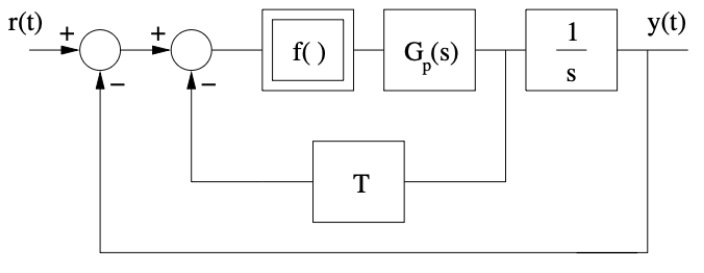
\includegraphics[width=\textwidth]{img/uklad.png}
        \caption{Schemat symulowanego układu gdzie $G_p = \frac{k+p}{1+T_ps}$}
    \end{minipage}\hfill
    \begin{minipage}{0.45\textwidth}
        \centering
        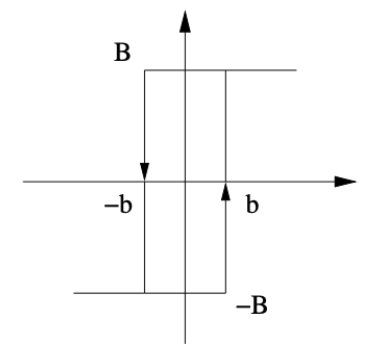
\includegraphics[width=\textwidth]{img/histereza.png}
        \caption{Charakterystyka elemntu nieliniowego $f()$ z symulowanego układu}
    \end{minipage}
\end{figure}

\section{Część teoretyczna}
Układ nieliniowy, który symulowaliśmy, składa się z elementu liniowego oraz elementu nieliniowego opisanego funkcją $f()$,
która posiada charakterystykę histerezową. Element liniowy jest typowym układem pierwszego rzędu, natomiast element nieliniowy wprowadza do układu nieliniowość, co powoduje,
że odpowiedź układu na sygnały wejściowe jest bardziej złożona i może wykazywać różne zachowania w zależności od parametrów układu i sygnałów wejściowych.

\smallbreak

Zaczęto od nazwania wszystkich sygnałów w układzie: \\
\begin{align*}
    r(t) &- \text{sygnał wejściowy}\\
    e(t) &- \text{uchyb sterowania}\\
    e_1(t) &- \text{sygnał wejściowy histerezy}\\
    u(t) &- \text{sygnał wyjściowy histerezy}\\
    x_2(t) &- \text{sygnał wejściowy elementu liniowego}\\
    x_1(t) &- \text{sygnał wyjściowy układu}
\end{align*}
Następnie wyznaczono zależności między sygnałami w układzie.
\begin{align*}
    e(t) &= r(t) - x_1(t) \\
    e_1(t) &= e(t) - T \cdot x_2(t) \\
    u(t) &= \begin{cases}
        -B \text{ dla } e_1(t) < -b \\
        B \text{ dla } e_1(t) > b \\
        u(t-1) \text{ dla } -b \leq e_1(t) \leq b
    \end{cases}\\
    X_2(s) &= \frac{k_p}{1+T_ps} \cdot U(s) \\
    X_1(s) &= \frac{1}{s} \cdot X_2(s)
\end{align*}
Co po przekształceniach daje poniższy układ równań różniczkowych opisujący zachowanie układu nieliniowego:
\begin{gather*}
    u(t) = \begin{cases}
        -B \text{ dla } r(t) - x_1(t) - Tx_2(t) < -b \\
        B \text{ dla } r(t) - x_1(t) - Tx_2(t) > b \\
        u(t-1) \text{ dla } -b \leq r(t) - x_1(t) - Tx_2(t) \leq b
    \end{cases} \\
    \begin{cases}
        \dot{x_1}(t) = x_2(t) \\
        \dot{x_2}(t) = -\frac{1}{T_p} \cdot x_2(t) + \frac{k_p}{T_p} \cdot u(t)
    \end{cases}
\end{gather*}
Przekształcenie problemu do postaci rówań różniczkowych pozwoliło na zastosowanie szeregu metod numerycznych do symulacji działania układu.
W celu osiągnięcia maksymalnej dokładności postanowiono zastosować metodę Rungego-Kutty czwartego rzędu z adaptacyjnym krokime symulacji.
Do tego celu wykorzystano metodę Dormanda-Prince'a, opisaną poniższą tabelą Butchera:
\begin{table}[h]
    \centering
    \begin{tabular}{c|ccccccc}
    0 & 0 & 0 & 0 & 0 & 0 & 0 & 0 \\
    $\frac{1}{5}$ & $\frac{1}{5}$ & 0 & 0 & 0 & 0 & 0 & 0 \\
    $\frac{3}{10}$ & $\frac{3}{40}$ & $\frac{9}{40}$ & 0 & 0 & 0 & 0 & 0 \\
    $\frac{4}{5}$ & $\frac{44}{45}$ & $-\frac{56}{15}$ & $\frac{32}{9}$ & 0 & 0 & 0 & 0 \\
    $\frac{8}{9}$ & $\frac{19372}{6561}$ & $-\frac{25360}{2187}$ & $\frac{64448}{6561}$ & $-\frac{212}{729}$ & 0 & 0 & 0 \\
    1 & $\frac{9017}{3168}$ & $-\frac{355}{33}$ & $\frac{46732}{5247}$ & $\frac{49}{176}$ & $-\frac{5103}{18656}$ & 0 & 0 \\
    1 & $\frac{35}{384}$ & 0 & $\frac{500}{1113}$ & $\frac{125}{192}$ & $-\frac{2187}{6784}$ & $\frac{11}{84}$ & 0 \\
    \hline
    & $\frac{35}{384}$ & 0 & $\frac{500}{1113}$ & $\frac{125}{192}$ & $-\frac{2187}{6784}$ & $\frac{11}{84}$ & 0 \\
    & $\frac{5179}{57600}$ & 0 & $\frac{7571}{16695}$ & $\frac{393}{640}$ & $-\frac{92097}{339200}$ & $\frac{187}{2100}$ & $\frac{1}{40}$
    \end{tabular}
    \caption{Tabela Butchera dla metody Dormanda-Prince'a}
\end{table}
Wykorzystując te współczynniki obliczono kolejne paramtery $k_i$, a później wyniki 5-tego i 4-tego rzędu. W ten sposób otrzymano po dwie estymacje dla obu zmiennych $x_1$ oraz $x_2$.
Obliczono błędy estymacji dla obu zmiennych poprzez porównanie wyników 5-tego i 4-tego rzędu, a następnie znormalizowane je względem tolerancji względnej i bezwzględnej wykorzystując wzór:
\begin{equation*}
    \text{err}_{\text{norm}} = \frac{\text{error}}{\text{tol}_{\text{abs}} + \text{tol}_{\text{rel}} \cdot \max(|x^{(5)}(t+h)|, |x(t)|)}
\end{equation*}
Ten sposób normalizaji unika problemów z dzieleniem przez zero w przypadku gdy $x(t)$ zbliża się do zera. Wybieramy także większą wartość pomiędzy estymacją a aktualną wartością, by zwiększyć
stabilność w przypadku gwałtownych zmian w sygnale. Następnie na podsawie największego z dwóch znormalizowynch błedów dopuszczamy lub odrzucamy krok symulacji, a także dostosowujemy jego długość do aktualnej sytuacji w układzie.
W celu osiągnięcia lepszej dokładności oraz zapobiegnięcia zatrzymania się symulacji dodano również maksymalną i minimalną długość kroku symulacji, a także maksymalną ilość iteracji.

Do wyznaczaniena następnej długości kroku symulacji wykorzystano wzór:
\begin{equation*}
    h_{\text{next}} = s \cdot h \cdot (\frac{1}{\text{err}_{\text{norm}}})^{\frac{1}{5}}
\end{equation*}
gdzie $s$ jest współczynnikiem bezpieczeństwa, a $h$ poprzednią długością kroku.

W przypadku gdy krok jest akcpetowany wykorzystywana jest estymacja 5-tego rzędu, uznawana za bardziej dokładną.

\section{Implementacja programu}
TODO: Implementacja

\section{Wyniki symulacji}
TODO: Wyniki symulacji(screeny)

\section{Wnioski}
TODO: Wnioski
\end{document}
